\documentclass[11pt]{article}
\usepackage{qlta}

\pgfplotsset{compat=1.18}

% Setup Tikz
\usetikzlibrary{positioning}
\usetikzlibrary{decorations.text}
\tikzstyle{inputNode}=[draw,circle,minimum size=10pt,inner sep=0pt]
\tikzstyle{stateTransition}=[-stealth, thick]

\title{Foundation of Machine Learning}
\subtitle{Chapter 1: Probabilistic Formulations of Prediction Problems}
\classinfo{Thursday, September 21, 2023}
\lecturer{Prof. Atif Jamal}
\studentone{EL HITARY Doha}
\studenttwo{TA Quyen Linh}

\begin{document}

    \maketitle
    \tableofcontents
    \vspace{5mm}
% \linenumbers


    \section{Introduction}

    \textit{Artificial Intelligence} (\textbf{AI}), originating from the core concepts of cybernetics, illustrates how comprehending intricate systems and regulatory methods led to the birth of artificial constructs exhibiting intelligent actions.

    The inaugural discourse on AI can be traced back to the 1950s with pioneers like \textit{Alan Turing}\footnote{Alan Turing (1912-1954) was a British mathematician, logician, and computer scientist often considered the father of computer science and artificial intelligence. He is best known for his work on breaking the German Enigma codes during World War II and for the Turing test, a criterion for whether a machine can be considered intelligent.} and \textit{John von Neumann}\footnote{John von Neumann (1903-1957) was a Hungarian-American mathematician, physicist, and computer scientist who made significant contributions to a vast range of fields. Notably, he laid the foundational framework for the architecture of modern digital computers with his von Neumann architecture, which described a computing device with data and programs stored in the same memory space.} examining the potential of intelligent machinery. Their motivations stemmed from desires to tackle intricate mathematical challenges and emulate human cognitive functions.

    Over the decades, AI has evolved from rule-based systems to data-driven approaches. The development of symbolic AI in the early years was followed by the advent of statistical AI and later, machine learning, which allowed systems to learn from data rather than relying solely on predefined rules.

    \paragraph{Machine Learning}A subfield of AI, heavily relies on the inductive principle to build models and make predictions. This approach allows machine learning systems to improve from experience and data collected over time. Induction, as a fundamental process, involves generalizing from specific data. It is the engine that enables algorithms to identify patterns, trends, and general rules from the provided data.

    For these rules to emerge robustly, having a sufficient amount of data and a representative sample is essential. Sample representativeness is controlled using statistics and probabilities. For instance, bounds can be defined to limit errors and ensure that samples effectively capture the inherent variability in the data, which is crucial for obtaining reliable and accurate Machine Learning models.

    Since the 2000s, there has been a true explosion of data that profoundly impacted the field of Machine Learning, giving rise to a strongly data-driven approach.

    The advent of the internet, social networks, connected sensors, and other sources of digital data led to exponential growth in available information. This abundance of data opened new possibilities and challenges for Machine Learning. The scale of massive data, commonly referred to as \textit{Big Data}, required the development of specific techniques and infrastructures for storing, processing, and extracting useful information. Machine Learning was particularly beneficial in this context as it allowed for the rapid analysis of vast amounts of data to extract patterns, trends, and valuable insights.

    Another approach in artificial intelligence emerged in the 1940s, known as \textit{connectionism}. Its origins trace back to the work of \textit{Warren McCulloch}\footnote{Warren McCulloch (1898-1969) was an American neurophysiologist and cybernetician who made foundational contributions to understanding the brain and its neural networks.} and \textit{Walter Pitts}\footnote{Walter Pitts (1923-1969) was a logician who worked with Warren McCulloch to develop early models of neural networks and neural computation.}, who proposed a simplified mathematical model of biological neurons. However, connectionism truly gained momentum in the 1950s and 1960s with the development of the first artificial neural networks, such as \textit{Frank Rosenblatt}'s \textit{perceptron}\footnote{Frank Rosenblatt (1928-1971) was an American psychologist and computer scientist, best known for inventing the perceptron, a type of artificial neural network.}.

    In the subsequent decades, connectionism experienced highs and lows, with periods of stagnation, notably in the 1970s and 1980s. However, it underwent a spectacular resurgence starting from the 2000s, thanks to increased computing power and data abundance. It was during this time that the term \textit{Deep Learning} was popularized to describe deep neural networks characterized by multiple hidden layers. Thus, connectionism evolved over the decades to become Deep Learning, a powerful approach that revolutionized various fields, from image recognition to automatic translation and natural language understanding. This transformation was fueled by algorithmic advancements, sophisticated neural network architectures, and the data explosion, making Deep Learning one of the most influential technologies of our time.

    \paragraph{Fundamentals of Backpropagation in Deep Learning} In deep learning, the learning rule of neurons is essential for allowing a neural network to adjust and learn from data. One of the primary learning mechanisms in neural networks is backpropagation of the gradient, often simply referred to as backpropagation. This technique is used to adjust the weights between neurons to optimize the network's performance.

    Backpropagation is an iterative process that starts with feeding a training data point into the network. The weights of the connections between neurons are initially assigned randomly or through specific initialization. When data is propagated through the network, each neuron performs a linear combination of inputs weighted by connection weights and then applies an activation function to produce its output.

    \begin{figure}[ht]
        \centering
        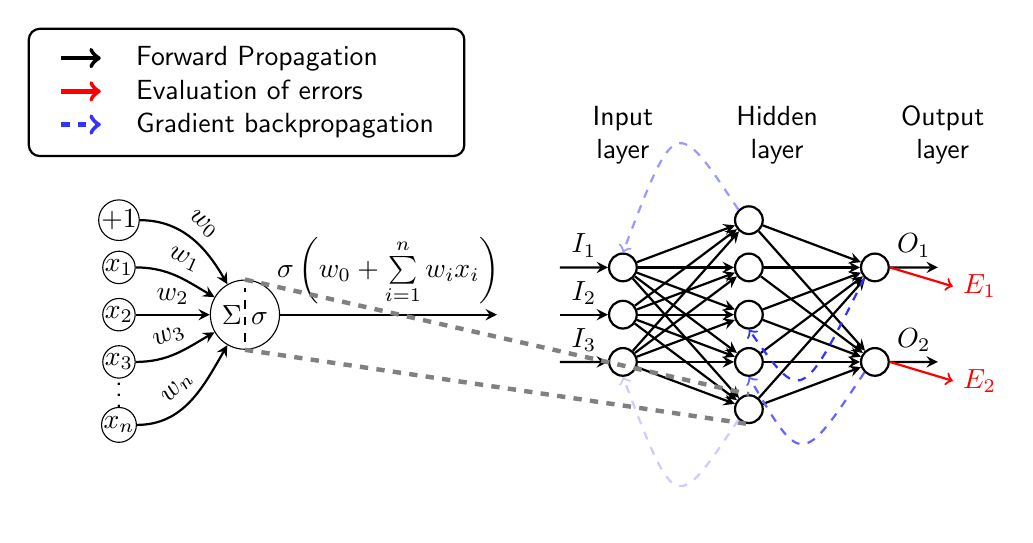
\begin{tikzpicture}[scale=0.8, font=\sffamily]
            \node[draw,circle,minimum size=25pt,inner sep=0pt] (x) at (0,0) {$\Sigma$ $\sigma$};

            \node[inputNode] (x0) at (-2, 1.5) {$\tiny +1$};
            \node[inputNode] (x1) at (-2, 0.75) {$\tiny x_1$};
            \node[inputNode] (x2) at (-2, 0) {$\tiny x_2$};
            \node[inputNode] (x3) at (-2, -0.75) {$\tiny x_3$};
            \node[inputNode] (xn) at (-2, -1.75) {$\tiny x_n$};

            \draw[stateTransition] (x0) to[out=0,in=120] node [midway, sloped, above] {$w_0$} (x);
            \draw[stateTransition] (x1) to[out=0,in=150] node [midway, sloped, above] {$w_1$} (x);
            \draw[stateTransition] (x2) to[out=0,in=180] node [midway, sloped, above] {$w_2$} (x);
            \draw[stateTransition] (x3) to[out=0,in=210] node [midway, sloped, above] {$w_3$} (x);
            \draw[stateTransition] (xn) to[out=0,in=240] node [midway, sloped, above] {$w_n$} (x);
            \draw[stateTransition] (x) -- (4,0) node [midway,above] {$\sigma\left(w_0 + \sum\limits_{i=1}^{n}{w_ix_i}\right)$};
            \draw[dashed] (0,-0.43) -- (0,0.43);
            \node (dots) at (-2, -1.15) {$\vdots$};
            \node[inputNode, thick] (i1) at (6, 0.75) {};
            \node[inputNode, thick] (i2) at (6, 0) {};
            \node[inputNode, thick] (i3) at (6, -0.75) {};

            \node[inputNode, thick] (h1) at (8, 1.5) {};
            \node[inputNode, thick] (h2) at (8, 0.75) {};
            \node[inputNode, thick] (h3) at (8, 0) {};
            \node[inputNode, thick] (h4) at (8, -0.75) {};
            \node[inputNode, thick] (h5) at (8, -1.5) {};

            \node[inputNode, thick] (o1) at (10, 0.75) {};
            \node[inputNode, thick] (o2) at (10, -0.75) {};

            \draw[stateTransition] (5, 0.75) -- node[above] {$I_1$} (i1);
            \draw[stateTransition] (5, 0) -- node[above] {$I_2$} (i2);
            \draw[stateTransition] (5, -0.75) -- node[above] {$I_3$} (i3);

            \draw[stateTransition] (i1) -- (h1);
            \draw[stateTransition] (i1) -- (h2);
            \draw[stateTransition] (i1) -- (h3);
            \draw[stateTransition] (i1) -- (h4);
            \draw[stateTransition] (i1) -- (h5);
            \draw[stateTransition] (i2) -- (h1);
            \draw[stateTransition] (i2) -- (h2);
            \draw[stateTransition] (i2) -- (h3);
            \draw[stateTransition] (i2) -- (h4);
            \draw[stateTransition] (i2) -- (h5);
            \draw[stateTransition] (i3) -- (h1);
            \draw[stateTransition] (i3) -- (h2);
            \draw[stateTransition] (i3) -- (h3);
            \draw[stateTransition] (i3) -- (h4);
            \draw[stateTransition] (i3) -- (h5);

            \draw[stateTransition] (h1) -- (o1);
            \draw[stateTransition] (h1) -- (o2);
            \draw[stateTransition] (h2) -- (o1);
            \draw[stateTransition] (h2) -- (o2);
            \draw[stateTransition] (h3) -- (o1);
            \draw[stateTransition] (h3) -- (o2);
            \draw[stateTransition] (h4) -- (o1);
            \draw[stateTransition] (h4) -- (o2);
            \draw[stateTransition] (h5) -- (o1);
            \draw[stateTransition] (h5) -- (o2);

            \node[above=of i1, align=center] (l1) {Input \\ layer};
            \node[right=2.3em of l1, align=center] (l2) {Hidden \\ layer};
            \node[right=2.3em of l2, align=center] (l3) {Output \\ layer};

            \draw[stateTransition] (o1) -- node[above] {$O_1$} (11, 0.75);
            \draw[stateTransition] (o2) -- node[above] {$O_2$} (11, -0.75);

            \path[dashed, double, ultra thick, gray] (x.north) edge[bend left=0] (h5.north);
            \path[dashed, double, ultra thick, gray] (x.south) edge[bend right=0] (h5.south);

            \draw[->, thick, red] (o1.east) -- ++(1,-0.3) node[right] {$E_1$};
            \draw[->, thick, red] (o2.east) -- ++(1,-0.3) node[right] {$E_2$};

            \draw[->, thick, blue!80!white, dashed] (o1.south west) .. controls ++(-1,-2) .. (h3.south);
            \draw[->, thick, blue!60!white, dashed] (o2.south west) .. controls ++(-1,-1.5) .. (h4.south);
            \draw[->, thick, blue!40!white, dashed] (h1.north west) .. controls ++(-1,1.5) .. (i1.north);
            \draw[->, thick, blue!20!white, dashed] (h5.south west) .. controls ++(-1,-1.5) .. (i3.south);

            \node[draw, rectangle, thick, rounded corners, fill=white, anchor=south east, inner sep=5pt] at (3.5,2.5) {
                \begin{tabular}{cl}
                    \raisebox{2pt}{\tikz\draw[->, ultra thick, black] (0,0) -- (.5,0);}                 & Forward Propagation      \\
                    \raisebox{2pt}{\tikz\draw[->, ultra thick, red] (0,0) -- (.5,0);}                   & Evaluation of errors     \\
                    \raisebox{2pt}{\tikz\draw[->, ultra thick, blue!80!white, dashed] (0,0) -- (.5,0);} & Gradient backpropagation \\
                \end{tabular}
            };

        \end{tikzpicture}
        \caption{We can see that the learning rule of neurons in deep learning relies on the backpropagation of the gradient, which adjusts the weights between neurons so that the network can learn to optimally represent complex relationships between data by minimizing a predefined cost function. This learning rule allows neural networks to adapt to the underlying patterns in the data and generalize their knowledge to make accurate predictions on new, unseen data.}
    \end{figure}

    Once the network's output is generated for a given training data point, the error between the actual output and the expected output/ground-truth is calculated using a cost function. This error is then backpropagated through the network using the gradient of the cost function with respect to the weights. Backpropagation involves calculating how each weight should be adjusted to minimize the error, using gradient descent or its variants like stochastic gradient descent (SGD).

    The weights are then updated proportionally to the derivative of the cost function with respect to each weight, with a learning rate controlling the magnitude of updates. This weight update occurs iteratively for many training data points, and the process repeats over multiple training epochs to allow the network to converge to a state where it minimizes the error on the training data.

    Deep Learning has seen remarkable applications in various fields, including computer vision, natural language processing, and autonomous robotics. Its ability to automatically extract hierarchical features from data has revolutionized the way we approach complex problems.

    \paragraph{Machine Learning Paradigms}
    \begin{itemize}
        \item Supervised Learning:
        In supervised learning, given a dataset of input-output pairs, $(x_i, y_i)$, where $x_i \in \mathcal{X}$ and $y_i \in \mathcal{Y}$, the goal is to learn a function $f: \mathcal{X} \rightarrow \mathcal{Y}$ that accurately maps inputs to outputs.

        \item Unsupervised Learning:
        Here, the dataset consists only of inputs, $x_i \in \mathcal{X}$, without paired outputs. The objectives can range from clustering similar inputs together to reducing data dimensionality or modeling the data's underlying distribution.

        \item Reinforcement Learning:
        This involves an agent interacting with an environment to maximize a cumulative reward. The agent follows a policy $\pi: \mathcal{S} \rightarrow \mathcal{A}$, which maps states $s \in \mathcal{S}$ to actions $a \in \mathcal{A}$.

        \item Self-Supervised Learning:
        A variant of supervised learning, where labels are automatically generated from the input data itself. This is often used for model pre-training.
    \end{itemize}


    \section{Supervised Learning}

    In supervised learning, the primary objective is to develop a model that can make accurate predictions based on given observations. This process can be formally described as follows:

    Given an observation $x$ from a feature space $\mathcal{X}$, the goal is to predict an outcome $y$ that belongs to a set $\mathcal{Y}$ of possible outcomes. The feature space $\mathcal{X}$ represents all possible observations, while $\mathcal{Y}$ encompasses all potential outcomes or responses.

    \begin{example}
        Consider the scenario where $x$ represents a word in a document or an image. In this context, $y$ would correspond to the category of the document or the classification of the image.
    \end{example}

    To formalize the prediction process, we introduce a function, or hypothesis, denoted by $h(x)$. This function maps an observation $x$ to a predicted outcome, providing us with $h(x)$ as the prediction of $y$ based on $x$.

    In practice, the development of this predictive model is guided by data. Specifically, we use a dataset consisting of $n$ pairs:
    $$
    (x_1, y_1), (x_2, y_2), \dots, (x_n, y_n)
    $$
    Each pair in this dataset represents a known observation and its corresponding true outcome. Using this dataset, we aim to choose or train a function $h : \mathcal{X} \rightarrow \mathcal{Y}$ such that, when presented with a new observation $x$, $h(x)$ provides a prediction that is close to the true outcome $y$.

    But how do we quantify the accuracy or quality of our predictions? This brings us to the concept of a loss function. The \textit{loss function}, denoted by $l$, measures the discrepancy or \textit{loss} between the predicted outcome and the actual outcome. Formally, for a given prediction $h(x)$ and true outcome $y$, the loss is given by $l(y, h(x))$. This function provides a metric that quantifies the cost or penalty of predicting $h(x)$ when the true outcome is $y$. Ideally, we want this loss to be minimal, indicating that our predictions are accurate and reliable.

    \begin{example}
        In the pattern classification (binary classification), the loss function can be defined as:
        \begin{equation}
            l(y, h(x)) = \mathbbm{1}_{\{y \neq h(x)\}} \Longleftrightarrow
            l(y, h(x)) = \begin{cases}
                             0 & \text{ if } y = h(x) \\
                             1 & \text{ if } y \neq h(x)
            \end{cases}
        \end{equation}
        where $\mathbbm{1}_{\{ \cdot \}}$ is the indicator function that equals $1$ if the condition inside the braces is true, and $0$ otherwise.

        For regression problems, with $\mathcal{Y} = \mathbb{R}$, we could define the loss function as:
        \begin{equation}
            l(y, h(x)) = (y - h(x))^2
        \end{equation}
        This is also known as the quadratic loss function.
    \end{example}

    \subsection{Probabilistic Assumptions}

    We assume the first thing that the existence of a joint probability distribution, denoted by $P$, over the feature space $\mathcal{X}$ and the outcome space $\mathcal{Y}$. This distribution governs the generation of data points and their corresponding outcomes.

    On the other hand, the data pairs, $(X_1, Y_1), \dots, (X_n, Y_n)$, are considered to be samples drawn independently from the distribution $P$ (\textit{i.i.d}). This means that each data point is generated without any influence from other data points, and all data points adhere to the same distribution.

    Given these assumptions, the primary objective in supervised learning is to select a function \( h : \mathcal{X} \rightarrow \mathcal{Y} \) that minimizes the risk or expected loss. The risk of a hypothesis \( h \) is defined:
    \begin{equation}
        R(h) = \mathbb{E}_{(x, y) \sim P}[l(y, h(x))]
    \end{equation}
    Here, the expectation is computed with respect to the joint distribution \( P \).

    As a practical illustration, consider the case of binary classification. The risk, in this context, represents the misclassification probability:

    \begin{equation}
        R(h) = \mathbb{E}_P[\mathbbm{1}_{y \neq h(x)}] = \int_{\mathcal{X}} \int_{\mathcal{Y}} \mathbbm{1}_{y \neq h(x)} P(y|x) dP(x) dy
    \end{equation}

    Here:
    \begin{itemize}
        \item \( \mathbbm{1}_{y \neq h(x)} \) is the indicator function, taking the value 1 when \( y \) is not equal to \( h(x) \) and 0 otherwise.
        \item The integral term represents the overall probability of misclassification across the feature and outcome spaces.
    \end{itemize}

    \begin{remark}
        We have some following points:
        \begin{itemize}
            \item Capital letters $X$ and $Y$ are used to denote random variables, while lower case letters $x$ and $y$ are used to denote their values.
            \item $P$ models both the relative frequency of different features $\mathcal{X}$ and the relationship between the features and the labels $\mathcal{Y}$.
            \item The assumption that the samples are i.i.d. is very strong.
            \item The function \(x \mapsto h_n(x : X_1, Y_1, \dots, X_n, Y_n)\) is random, since it depends on the random samples \(D_n = \{(X_1, Y_1), \dots, (X_n, Y_n)\}\).
        \end{itemize}
    \end{remark}

    Given this understanding, the risk associated with a hypothesis can be described as:
    \begin{equation}
        h_n = \mathbb{E}_{P}[l(y, h_n(x))] = \mathbb{E}[l(Y_1, h_n(X_1)) + \cdots + l(Y_n, h_n(X_n)) \mid D_n]
    \end{equation}
    Our objective in supervised learning is often to ensure that the expected risk $\mathbb{E}[R(h_n)]$ is minimized. Alternatively, we may aim for the risk $R(h_n)$ to be small with a high probability across different realizations of the training sets $D_n$.

    \begin{figure}[h]
        \centering
        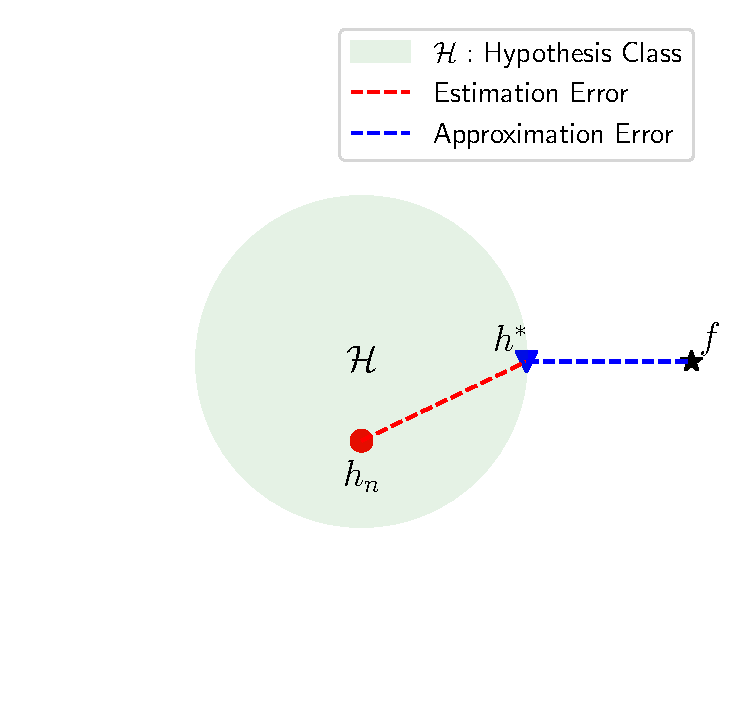
\includegraphics[trim=0.5cm 3cm 0.2cm 0.5cm, clip, width=8cm]{figures/fig1.1.pdf}
        \caption{For simply imagine, in this figure, we denote $h^*$ as the best function we could choose from the hypothesis space $\mathcal{H}$. The risk at $h^*$ is noted $\inf_{h \in \mathcal{H}} R(h)$. The true risk $\inf_{f} R(f)$ found outside $\mathcal{H}$.}
        \label{fig:risk_class}
    \end{figure}

    \begin{example}
        Examples of hypothesis classes, consider the domain $\mathcal{X}=\mathbb{R}^q$, a straightforward class is the set of linear functions, given by $f(x) = w^{\top}x + b$, where $w \in \mathbb{R}^q$ and $b \in \mathbb{R}$. Pushing the boundaries of linearity, we could leverage a nonlinear transformation $\psi: \mathcal{X} \rightarrow \mathbb{R}^E$. This leads to models like $f(x)=w^{\top}\psi(x) + b$, which, although linear in the transformed space $\mathbb{R}^E$, can encapsulate complex nonlinear dynamics in the original space $\mathcal{X}$. An illustrative transformation for a two-dimensional input might be $\psi(x) = [x_1, x_2, x_1^2, x_1x_2, x_2^2]^{\top}$, allowing the model to discern quadratic interactions and dependencies.
    \end{example}

    \subsection{Key Questions}

    In the realm of supervised learning, we often select our hypothesis function $h_n$ from a predefined class of functions, denoted as $\mathcal{H}$. This class could encompass a variety of models, ranging from linear classifiers to more complex structures like neural networks and decision trees. When navigating this landscape, several pivotal questions arise:

    \begin{enumerate}
        \item \textit{Optimality within Class:} Given that we've chosen our hypothesis from $\mathcal{H}$, can we design an algorithm such that the risk $R(h_n)$ is close to the best possible within this class? Formally, we desire $R(h_n) - \inf_{h \in \mathcal{H}} R(h)$ to be small.

        \item \textit{Dependency on Data:} How does the efficacy of our chosen $h_n$ relate to the size of our training dataset, denoted as $n$? Furthermore, how does the complexity of the function class $\mathcal{H}$ influence this performance?

        \item \textit{Global Optimality:} Beyond just our chosen class $\mathcal{H}$, can we ensure that our hypothesis $h_n$ approaches the globally optimal performance, represented as:
        $\inf_{f} R(f) \text{ ?}$
    \end{enumerate}

    \subsection{Key Issues}

    \begin{itemize}
        \item \textit{Approximation:} The first challenge pertains to the inherent capability of our chosen class $\mathcal{H}$. Specifically, we need to ascertain:
        $
        \inf_{h \in \mathcal{H}} R(h) - \inf_{f} R(f),
        $
        which quantifies how the best function in $\mathcal{H}$ compares to the globally optimal function.

        \item \textit{Estimation:} Once we've chosen a function from $\mathcal{H}$, the next challenge is to determine how well it performs relative to the best function in $\mathcal{H}$:
        $
        R(h_n) - \inf_{h \in \mathcal{H}} R(h).
        $

        \item \textit{Computation:} We need to use data to choose $h_n$ from $\mathcal{H}$, typically by slowing some kind of optimization problem. How can we do this efficiently?
    \end{itemize}

    \begin{figure}[h]
        \centering
        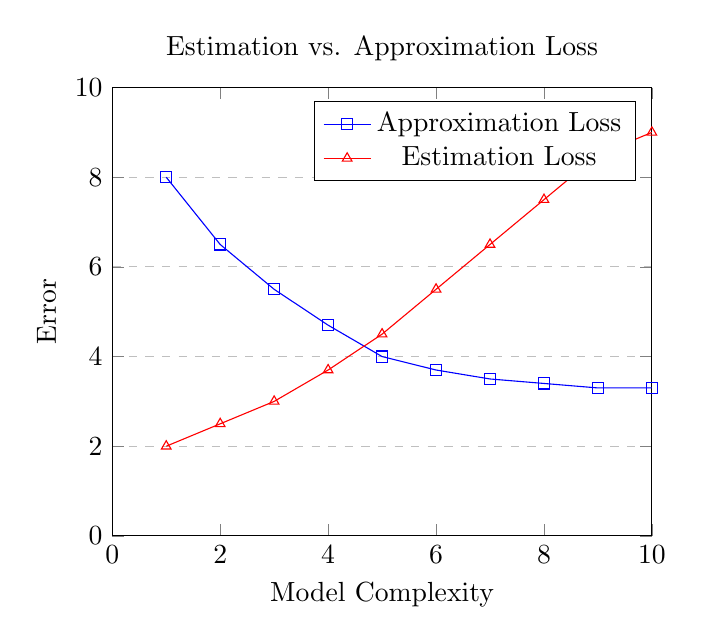
\begin{tikzpicture}
            \begin{axis}[
                title={Estimation vs. Approximation Loss},
                xlabel={Model Complexity},
                ylabel={Error},
                xmin=0, xmax=10,
                ymin=0, ymax=10,
                legend pos=north east,
                ymajorgrids=true,
                grid style=dashed,
            ]
                \addplot[
                    color=blue,
                    mark=square,
                ]
                coordinates {
                    (1,8)(2,6.5)(3,5.5)(4,4.7)(5,4)(6,3.7)(7,3.5)(8,3.4)(9,3.3)(10,3.3)
                };
                \addlegendentry{Approximation Loss}
                \addplot[
                    color=red,
                    mark=triangle,
                ]
                coordinates {
                    (1,2)(2,2.5)(3,3)(4,3.7)(5,4.5)(6,5.5)(7,6.5)(8,7.5)(9,8.5)(10,9)
                };
                \addlegendentry{Estimation Loss}
            \end{axis}
        \end{tikzpicture}
        \caption{Graph illustrating the trade-off between Estimation and Approximation Loss as model complexity increases. The blue curve (Approximation Loss) shows that as the model becomes more complex, it better approximates the underlying data distribution, hence the error decreases. However, after a certain point, the error plateaus, indicating that increasing complexity doesn't provide significant benefits. The red curve (Estimation Loss) indicates that simpler models generalize better, but as complexity increases, the models tend to overfit, leading to higher estimation errors. The optimal model complexity lies where the sum of these two errors is minimized.}
        \label{fig:est-app}
    \end{figure}

\end{document}
